% !TeX encoding = UTF-8
% !TeX spellcheck = de_DE

\documentclass[biblatex]{lni}
\addbibresource{lni-paper-example-de.bib}


\usepackage{booktabs} % Schöne Tabellen mittels \toprule, \midrule, \bottomrule
\usepackage[]{blindtext} % Zu Demonstrationszwecken
\usepackage{fancyhdr}
\usepackage{acronym}
\usepackage{hyperref}

%% Sietenzahlen
\pagestyle{fancy}
\fancyhf{}
\fancyfoot[C]{\thepage}
\renewcommand{\headrulewidth}{0pt}

\begin{document}

\begin{titlepage}
  \centering
  \vspace*{0.5cm}

  {\scshape\LARGE Fallstudie \par}

  {\huge\bfseries
    Analyse von Web Applikations-Technologien:
  \par
  }
  {\Large\itshape Am Beispiel der Planung einer GLS Quiz App\par}

  \vspace{1cm}

  {\Large\textbf{Eingereicht von: }}\\
  Nicolas Fritz \\
  E-Mail: nicolasnoah.fritz@gls-germany.com

  \vspace{1cm}

  {\Large\textbf{Eingereicht bei: }}\\
  Hochschule Fulda \\
  Leipziger Straße 123 \\
  36037 Fulda \\
  Lehrperson: Prof. Dr. Brigit Bomsdorf

  \vspace{1cm}

  {\Large\textbf{Unternehmen: }}\\
  GLS Germany GmbH & Co. OHG \\
  Betreuung: Laura Alles, Patrick Weppler

  \vfill

  {\large \today\par}
\end{titlepage}

\tableofcontents
\listoffigures
\newpage

\section*{Abkürzungsverzeichnis}
\begin{acronym}[Bash]
  \acro{WebApp}{Webanwendung}
  \acro{GUI}{Graphical User Interface, also Benutzeroberfläche}
  \acro{HTML}{Hypertext Markup Language}
  \acro{CSS}{Cascading Style Sheets}
  \acro{JS}{JavaScript}
  \acro{SPA}{Single Page Application}
  \acro{TS}{TypeScript}
  \acro{CLI}{Command Line Interface}
  \acro{DOM}{Document Object Model}
  \acro{JSX}{JavaScript XML}
  \acro{API}{Application Programming Interface}
  \acro{REST}{Representational State Transfer}
  \acro{JSON}{JavaScript Object Notation}
\end{acronym}
\newpage

\section{Einleitung}
Diese Fallstudie mit dem Titel „Analyse von Web Applikations-Technologien: Am Beispiel der Planung einer GLS Quiz App“
wurde im Fachbereich Angewandte Informatik von Nicolas Fritz im Unternehmen GLS Germany GmbH & Co. OHG erstellt.
Die Betreuung im Unternehmen erfolgte durch Patrick Weppler für den technischen Teil und Laura Alles für den konzeptionellen Teil.
An der Hochschule wurde die Arbeit von Prof. Dr. Birgit Bomsdorf betreut.
Das Thema wird anhand des Fallbeispiels einer GLS Quiz App erläutert und analysiert.

\subsection{Hintergrund und Motivation}
Software wird zunehmend komplexer und enthält immer mehr Funktionen, von denen viele standardisiert und wiederkehrend sind.
Je größer das Projekt, desto schwieriger wird es, den Überblick zu behalten – insbesondere bei Webanwendungen,
die sich kontinuierlich weiterentwickeln und fortlaufend programmiert werden.
Um den Überblick zu bewahren, sind daher Konzepte notwendig, die eine Erweiterbarkeit sicherstellen.
Außerdem muss Software skalierbar und gleichzeitig effizient sein.

\\

Ein Beispiel für eine solche Webanwendung, folgend nur WebApp, ist die GLS-Quiz App.
Diese App dient dazu, neue duale Studenten, Auszubildende oder Mitarbeiter mit dem Unternehmen vertraut zu machen.
Sie basiert auf einer zuvor genutzten analogen Version, in der die Nutzer in die Rolle eines Paketboten schlüpfen,
Pakete ausliefern und dabei auf verschiedene Probleme stoßen, die sie durch das Beantworten von Fragen lösen müssen.

\\

Im Verlauf der Konzeptionierung und Umsetzung der App stellte sich heraus,
dass die ursprüngliche analoge Version aufgrund der gewählten Technologie stark vereinfacht werden musste
und die Weiterentwicklung nun deutlich erschwert ist.

\\

Daher benötigen wir eine Lösung,
die eine vorgegebene Struktur bietet und grundlegende Funktionen bereits integriert.
Gleichzeitig müssen einfache Erweiterungsmöglichkeiten gewährleistet sein.

\subsection{Ziel der Fallstudie}

\subsection{Methodik und Vorgehensweise}

\section{Technologieüberblick}
Um die Entwicklung einer WebApp wie der GLS Quiz App besser zu verstehen,
ist es wichtig, die zugrunde liegenden Technologien zu kennen.

\\

Im folgenden Abschnitt werden die Grundlagen geschaffen,
moderne Technologien aufgezeigt und verglichen.
Zusätzlich wird die Zusammenarbeit der wichtigsten Komponenten einer WebApp aufgezeigt.

\subsection{Überblick über moderne Webtechnologien}
\label{sec:moderne-webtechnologien}

Um eine WebApp oder Website zu verstehen oder entwickeln zu können, ist es wichtig, die zugrunde liegende Struktur zu kennen.
Eine wesentliche Unterscheidung ist dabei die zwischen Frontend und Backend.

Das Frontend bezeichnet hierbei den sichtbaren Teil einer WebApp, den der Nutzer direkt erleben kann. \cite{CMSRev}
Anders gesagt ist es das \ac{GUI} einer Anwendung.
Es umfasst alles, was auf dem Bildschirm angezeigt wird, einschließlich Gestaltung und Interaktion.
Das Frontend besteht aus den drei grundlegenden Technologien \ac{HTML}, \ac{CSS} und \ac{JS}.

Die Seite Time4Innovation \cite{T4I} beschreibt die drei Technologien wie folgt: \\
\textbf{\ac{HTML}} ist der grundlegende Aufbau einer Seite.
Es definiert die Struktur und den Inhalt. \\
\textbf{\ac{CSS}} ist für das Design zuständig.
Die mit \ac{HTML} definierten Elemente werden hiermit gestaltet, also zum Beispiel Farben, Schriftarten und Abstände. \\
\textbf{\ac{JS}} ist für die Interaktion zuständig.
Alles was nicht mittels \ac{HTML} und \ac{CSS} umgesetzt werden kann, wird mit \ac{JS} realisiert.

Ein Frontend für eine WebApp besteht typischerweise aus diesen 3 Technologien oder Abwandlungen dieser. \cite{CoU}
Der Grund dafür ist, dass der Browser nur diese Sprachen versteht und sie für die Benutzer interpretiert.
Das ist der Grund dafür, dass diese Sprachen auch als \texttt{clientseitige} Sprachen bezeichnet werden.

\\

Das Backend hingegen benutzt \texttt{serverseitige} Sprachen. \cite{CMSRev}
Es ist verantwortlich für die Verwaltung von Daten und Verarbeitung von Benutzerinteraktionen.
Dabei umfasst es den Server, der Anfragen vom Frontend entgegennimmt und verarbeitet,
sowie die Datenbank, die unter anderem zur Speicherung der Daten dient.

Die Sprachen variieren stark und sind abhängig von den Anforderungen der Anwendung.
Typische serverseitige Sprachen sind \textbf{Java}, \textbf{Python} oder \textbf{PHP}.
Eine Besonderheit besteht darin, dass auch \ac{JS} serverseitig verwendet werden kann.

\\

Doch wie bereits erwähnt reicht eine Sprache nicht aus, um eine WebApp zu entwickeln.
Heutige WebApps sind komplexer und benötigen daher sogenannte Frameworks.
Eine Definition der Rock the Prototype Seite lautet: \\
\begin{minipage}{\textwidth}
  \textit{
    \\
    \\
    \textbf{"} \\
    Frameworks bieten vorgefertigten Code,
    der als Ausgangspunkt für die Entwicklung von Anwendungen verwendet werden kann. Dies spart Zeit und Mühe,
    da die Entwickler nicht von Grund auf mit der Programmierung beginnen müssen.
    Stattdessen können sie den vorgefertigten Code als Grundlage verwenden und ihn mit eigenem Code ergänzen.
    \\
    \textbf{"} \\
    \Cite{RtP}
    \\
  }
\end{minipage}

Also bedeutet das,
dass Frameworks den Entwicklungsprozess durch die Bereitstellung von Standardlösungen und wiederverwendbarem Code beschleunigen.
Entwickler können auf diese vorgefertigten Komponenten zurückgreifen,
um wiederkehrende Aufgaben zu automatisieren und sich auf die individuellen Anforderungen ihrer WebApp zu konzentrieren.
Frameworks helfen dabei, die Komplexität zu bewältigen,
indem sie eine strukturierte Basis bieten, auf der Entwickler ihre spezifischen Funktionen aufbauen können.

Im folgenden Abschnitt werden wir 3 Frontend- und Backend-Frameworks etwas genauer betrachten und miteinander vergleichen.

\subsection{Frontend-Technologien im Vergleich: VueJS, Angular und React}

\begin{figure}
  \centering
  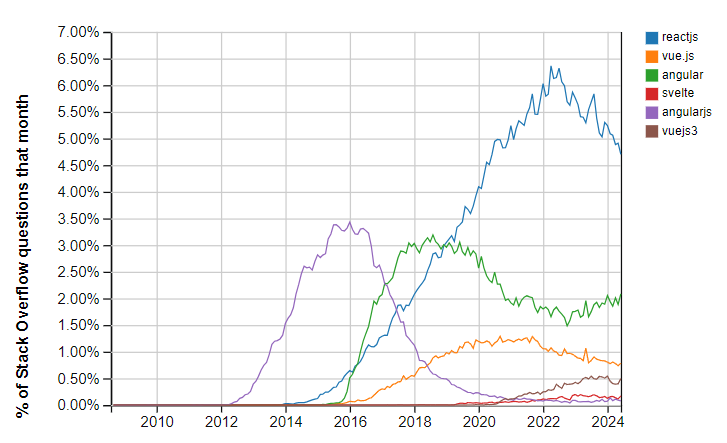
\includegraphics[width=.8\textwidth]{fetrends}
  \caption{Stackoverflow Fragen Frontend-Frameworks.}
  \label{fig:fetrends}
  \vspace{-0.3cm}
  \begin{center}
    \footnotesize Quelle: \cite{SOTrend}
  \end{center}
\end{figure}

\Cref{fig:fetrends} zeigt den Verlauf der Fragen zu Webtechnologien auf Stack Overflow,
einer sehr bekannten Plattform für Programmierfragen, über die relevanten Jahre.
Die Grafik bietet zwar keinen umfassenden Einblick in die Nutzung von Frameworks in Unternehmen,
liefert jedoch eine grobe Orientierung darüber, welche Technologien Entwickler auch privat verwenden und somit bevorzugen.

Für den Vergleich der Frontend-Frameworks beziehe ich mich auf bereits vorhandene Vergleiche von
entwickler.de und browserstack.com. \cite{BStack} \cite{Dev}
Zusätzlich werde ich die jeweiligen Dokumentationen der Frameworks heranziehen,
um detaillierte Informationen und aktuelle Entwicklungen zu berücksichtigen.

Alle 3 Frameworks sind Open-Source, also frei verfügbar und können von jedem genutzt und weiterentwickelt werden.

\subsubsection{Vue}
Vue.js wurde 2014 von Evan You entwickelt und ist das jüngste der 3 Frameworks. \cite{AmD}
Es basiert auf der Idee einer \ac{SPA}, also einer Anwendung, die nur eine Seite lädt und dann dynamisch aktualisiert. \cite{BStack}
Der Vorteil an einer solchen WebApp ist, dass sie schneller und flüssiger läuft, da nicht bei jedem Klick eine neue Seite geladen werden muss.
Es wurde entwickelt, um die besten Teilaspekte von Angular zu übernehmen und gleichzeitig die Komplexität zu reduzieren,
was in einem effizienten und leistungsstarken Tool endete.

Die neueste Version, Vue 3,
wurde 2020 veröffentlicht und bringt signifikante Verbesserungen und neue Funktionen mit sich. \cite{vue}
Vue 3 bietet eine verbesserte Leistung durch den neuen Compiler, ein Programm, welches deinen Code in JavaScript übersetzt und somit für den Browser verständlich macht.
Dieser Compiler analysiert den Code und optimiert ihn, um die Ausführung zu beschleunigen.
Zudem unterstützt Vue 3 die TypeScript-Integration besser, was die Typisierung und Wartung des Codes erleichtert.
\ac{TS} ist eine Programmiersprache, die auf JavaScript aufbaut und zusätzliche Funktionen wie Typisierung und Klassen bietet. \cite{ts}
Somit wird der Code sicherer und einfacher zu warten.

\Cref{fig:fetrends} lässt darauf schließen,
dass Vue mit Vue.js und Vue3 im Vergleich zu Angular und React weniger populär ist.
Dennoch ist es eindeutig auf Platz 3.
Zu erkennen ist ein Abfall der Fragen von VueJS und ein Anstieg von Vue 3, was den Versionswechsel verdeutlicht.
Dieser zieht sich aber eher hin und geht langsam voran.

Eines der Vorteile von vue ist, dass es eine sehr kurze Lernkurve hat. \cite{Dev}
Im Vergleich zu anderen Frameworks wie Angular oder React,
ist Vue sehr anfängerfreundlich und benötigt nicht viele Vorkenntnisse.
Trotzdem ist es sehr leistungsstark und kann auch für größere Projekte verwendet werden.
Außerdem ist Vue sehr klein und verhindert somit, dass die Seite lange zum Laden benötigt.
Heutzutage ist das ein sehr wichtiger Faktor, da zum Beispiel Google die Ladezeit einer Seite als Rankingfaktor verwendet. \cite{GLZ}

Ein schwerwiegender Nachteil ist jedoch, dass es im Vergleich zu anderen Frameworks weniger Support und weniger Entwickler gibt, wie bereits aus \Cref{fig:fetrends} entnommen. \cite{BStack}
So kann es dazu führen, dass die Unterstützung von älteren Versionen fehlt oder weniger Erweiterungen verfügbar sind.
Das kann dazu führen, dass manche Funktionen selbst entwickelt werden müssen, was Zeit und Geld kostet.
Zudem fehlt im Vergleich zu Angular und React die Unterstützung von großen Unternehmen, was die Verbreitung und Weiterentwicklung einschränkt.

\subsubsection{Angular}

In Bezug auf Angular und AngularJS zeigt \Cref{fig:fetrends} eine mittlere Beliebtheit.
Während AngularJS nach seiner Veröffentlichung große Aufmerksamkeit erregte,
insbesondere aufgrund seiner revolutionären Ansätze,
wurde der Nachfolger Angular ab 2019 von React überholt und ist seither nicht mehr die beliebteste Wahl.
Der Übergang von AngularJS zu Angular erfolgte jedoch schneller als der Wechsel von Vue zu Vue 3.
Seit 2023 ist ein Anstieg der Anzahl an Fragen zu Angular zu beobachten,
was auf ein wieder wachsendes Interesse an diesem Framework hindeutet.

Angular wurde von Google entwickelt und basiert auf \ac{TS}. \cite{NG}
Dabei ist es ein muss, TypeScript zu verwenden, da Angular kein JavaScript unterstützt.
Meist werden auch \ac{SPA}s mit Angular entwickelt werden, es ist jedoch auch möglich, mehrseitige Anwendungen zu erstellen.
Eine besonderheit stellt das \ac{CLI} dar, das es ermöglicht, schnell und einfach ein neues Projekt zu erstellen und zu verwalten.

Ein großer Vorteil von Angular ist, dass es sehr Zukunftssicher ist. \cite{BStack}
Dies kommt dadurch Zustande, da Google hinter dem Framework steht und es ständig weiterentwickelt.
Auch die Dokumentation ist sehr umfangreich und gut strukturiert, was die Einarbeitung erleichtert. \cite{NG}
Es eignet sich perfekt für große Projekt, da die Projektstruktur konsistenz und lesbarkeit fördert

Ein Nachteil ist jedoch, dass Angular sehr komplex ist und eine lange Einarbeitungszeit benötigt. \cite{BStack}
Dadurch ist es weniger für Anfänger geeignet und benötigt mehr Vorkenntnisse.
Auch die Ladezeit einer Seite ist länger, da Angular sehr groß ist und viele Funktionen mitbringt.
Bei großen WebApps spielt das weniger eine Rolle, aber bei kleinen WebApps ist das ein großer Nachteil.

\subsubsection{React}

Wie in \Cref{fig:fetrends} zu sehen ist, hat sich React seit seiner Einführung als besonders beliebt erwiesen.
Die stetig wachsende Anzahl der Fragen deutet auf eine wachsende Nutzerbasis hin.
Der Höhepunkt der Beliebtheit von React war 2022, seitdem fällt die Anzahl der Fragen.

React wurde 2013 von Facebook entwickelt und gehört seither zu den beliebtesten Frontend-Frameworks. \cite{BStack}
Wie Vue und Angular ist auch React für \ac{SPA}s geeignet und verwendet ein Baustein System, in dem Komponenten wiederverwendet werden können.
Ahnlich wie Vue3 kann React auch mit \ac{TS} verwendet werden.\cite{RCT}

Ein Vorteil von React ist die relativ einfache Lernkurve. \cite{BStack}
Zudem profitieren Entwickler von der großen Community und den zahlreichen Erweiterungen,
die viele Funktionen bereits vorgefertigt anbieten,
sodass sie nicht von Grund auf neu programmiert werden müssen.
Damit einher geht auch das React Ökosystem, zudem auch React-Native gehört und es ermöglicht,
auch mobile Apps zu entwickeln und somit den Code zu teilen. \cite{RCTN}

Mit dem Vorteil der Größe folgt jedoch auch ein Nachteil. \cite{BStack}
Durch die Größe und Beliebtheit von React ist das Tempo der Weiterentwicklung sehr hoch,
was Entwickler zwingt, sich ständig mit neuen Konzepten auseinanderzusetzen.
Zudem verwendet React \ac{JSX}, ein spezielles Format, um \ac{HTML} in JavaScript zu schreiben. \cite{JSX}
Für Anfänger kann \ac{JSX} ungewohnt sein und eine gewisse Einarbeitungszeit erfordern.

\subsection{Backend-Technologien im Vergleich: Express, Springboot und Django}

\subsubsection{Express}
\subsubsection{Springboot}
\subsubsection{Django}

\subsection{Wie arbeiten Backend und Frontend zusammen?}

\section{Die GLS Quiz App}
\subsection{Ist-Zustand der App}
\subsection{Ursprüngliches Konzept}
\subsection{Probleme bei der Umsetzbarkeit des ursprünglichen Konzepts}
\subsection{Konzeptentwicklung zur Bewältigung der Herausforderungen}

\section{Test-Implementierung}

Um das Verständnis zu vertiefen und die Bewertung der Technologien im Bezug auf die GLS-Quiz-App zu erleichtern,
wird in diesem Abschnitt ein Demo Projekt vorgestellt.
Der Fokus liegt zunächst auf einer allgemeinen Einführung,
gefolgt von einer detaillierten technischen Umsetzung.
Abschließend werden die gewonnenen Erkenntnisse aus der Implementierung dargelegt.

Das Hauptziel besteht darin,
aus allen Frontend- und Backend-Technologien die bestmögliche Kombination für die finale Lösung zu ermitteln.
Dazu wird ein Prototyp entwickelt, der mit allen bereits vorgestellten Frontend- und Backend-Technologien realisiert wird,
sowohl auf der Backend-Seite (Spring Boot, Express, Django) als auch auf der Frontend-Seite (Vue, Angular, React).

\subsection{Das Demo Projekt}

Das Demo-Projekt ist eine simple Fragen-App und simuliert damit auf einer sehr einfachen Ebene die GLS-Quiz-App.
Die App ist in zwei Hauptteile unterteilt: Frontend und Backend, wie in dem Abschnitt \hyperref[sec:moderne-webtechnologien]{\textit{Überblick über moderne Webtechnologien}} beschrieben.

Die Fragen-App stellt dem Nutzer nacheinander verschiedene Fragen,
die jeweils mehrere Antwortmöglichkeiten bieten \textit{(a, b, c)}.
Jede Frage hat genau eine richtige Antwort.
Der Nutzer kann eine Antwort auswählen und muss diese anschließend bestätigen.
Nach der Bestätigung erhält der Nutzer eine Rückmeldung,
ob seine Antwort richtig oder falsch war.
Es ist sicherzustellen, dass der Nutzer nicht durch Einsicht in den Quelltext der App die korrekten Antworten herausfinden kann.

Das Frontend ist ausschließlich für die visuelle Darstellung der App zuständig.
Es zeigt die Fragen, die Antwortmöglichkeiten und das Ergebnis der Beantwortung an.

Das Backend fungiert als \ac{REST}-\ac{API} und ist verantwortlich für die Bereitstellung der Fragen und die Überprüfung der Antworten.
Das Thema Datenbank ist zu vernachlässigen.
Stattdessen soll das Backend auf eine einfache Methode zurückgreifen, wie zum Beispiel die Verwendung einer einzelnen Datei.

\subsection{Umsetzung}

- gesamtes Projekt unter https://github.com/hypeAlive/fallstudie-impl.git

\subsubsection{Frontend}

- Läuft bei allen auf port 2400

\subsubsection{Backend}

- Läuft bei allen auf port 8080
- sendet und empfängt JSON
- Simulierte Datenbank in Form von JSON Datei, die von allen Backends geteilt wird
    - läd bei start einmal alle Fragen in das Backend, also wird nicht immer wieder neu geladen

- API Schnittstellen:

\textit{\textbf{GET} /type}, gibt den Typen des Backends zurück. \\
\begin{lstlisting}[caption={\ac{JSON} der Route \textbf{GET} /question/ids }, label=get-ids, language=typescript]
{
  "type": "express" | "spring" | "django" // Backend Typ
}
\end{lstlisting}

\textit{\textbf{GET} /question/ids}, gibt eine Liste aller ids in Form von Nummern zurück. \\
\begin{lstlisting}[caption={\ac{JSON} der Route \textbf{GET} /type }, label=type, language=typescript]
number[]
\end{lstlisting}

\textit{\textbf{GET} /question/\{id\}}, gibt eine Frage anhand id zurück. \\
\begin{lstlisting}[caption={\ac{JSON} der Route \textbf{GET} /question/\{id\} }, label=get-questionbyid, language=typescript]
{
  "id": number, // ID der Frage zur Identifikation
  "question": string // Die Frage
  "options": [
    {
      "type": "a" | "b" | "c", // Antwortmöglichkeiten
      "text": string // Text der Antwortmöglichkeit
    }
  ]
}
\end{lstlisting}

\textit{\textbf{GET} /question}, gibt eine Liste aller Fragen zurück. \\
\begin{lstlisting}[caption={\ac{JSON} der Route \textbf{GET} /question }, label=get-question, language=typescript]
[
  {
    ... //siehe /question/{id} Objekt
  },
  ...
]
\end{lstlisting}

\textit{\textbf{POST} /question}, gibt eine Fragen anhand id zurück. \\
\begin{lstlisting}[caption={Request \ac{JSON} der Route \textbf{POST} /question }, label=post-question-req, language=typescript]
{
  "id": number,
  "answer": "a" | "b" | "c"
}
\end{lstlisting}
\begin{lstlisting}[caption={Response \ac{JSON} der Route \textbf{POST} /question }, label=post-question-res, language=typescript]
{
  "id": number,
  "isCorrect": boolean // Ob die Antwort richtig war
}
\end{lstlisting}


\subsection{Ergebnisse und erlangtes Wissen}

\section{Schlussfolgerung und Ausblick}

\newpage
\section{Anhang}
\newpage
\printbibliography

\end{document}
